% @Author: soheilred
% @Date:   2018-10-28 01:10:54
% @Last Modified by:   soheilred
% @Last Modified time: 2018-12-10 15:37:25
\documentclass{beamer}

\let\val\undefined
\usepackage{pgf}
\usepackage{pgfplots}
\usepackage{tikz}
\usepackage{booktabs}
\usepackage{natbib}
\usepackage{framed}
\usepackage{longtable}
\usepackage{bigdelim,multirow}
\usepackage{amsmath}
\usepackage{amsthm}
\usepackage{mathtools}
\DeclareMathOperator{\argmax}{argmax} % no space, limits on side in displays


\usetikzlibrary{arrows,automata,backgrounds,positioning,decorations,intersections,matrix}

% *** Styles ***
\setbeamertemplate{navigation symbols}{}
\usecolortheme{dolphin}
%\usecolortheme{rose}
\setbeamercovered{transparent}
\usefonttheme{professionalfonts}
%\usefonttheme[onlymath]{serif}

% 
\addtobeamertemplate{navigation symbols}{}{%
    \usebeamerfont{footline} %
    \usebeamercolor[fg]{footline}%
    \hspace{1em}%
    \insertframenumber/\inserttotalframenumber
}

\DeclarePairedDelimiter{\norm}{\lVert}{\rVert}
\DeclarePairedDelimiter\abs{\lvert}{\rvert}%


% \setlist[itemize,1]{label=$\times$}
% \setlist[itemize,2]{label=$\checkmark$}
% \setlist[itemize,3]{label=$\diamond$}
% \setlist[itemize,4]{label=$\bullet$}


% *** Colors ***
\newcommand{\tc}[2]{\textcolor{#1}{#2}}
\newcommand{\tcb}[1]{\tc{blue}{#1}}
\newcommand{\tcr}[1]{\tc{red}{#1}}
\newcommand{\tcg}[1]{\tc{green}{#1}}

\def\checkmark{\tikz\fill[scale=0.4](0,.35) -- (.25,0) -- (1,.7) -- (.25,.15) -- cycle;} 

\newcommand{\Ex}{\mathbb{E}}
%\newcommand{\Pr}{\mathbb{P}}
\DeclareMathOperator{\Var}{Var}

\definecolor{varcolor}{RGB}{132,23,49}
\newcommand{\varname}[1]{\textcolor{varcolor}{\mathsf{#1}}}

\title{How to win the battle against Glossy Buckthorn using RL}
\date{}

\begin{document}
\begin{frame}
	\maketitle

\end{frame}
%=====================================%
\begin{frame}
	\frametitle{Problem Definition}
	\begin{itemize}
		\item Having the population and the seed bank in a 9 cell environment (a $3 \times3$ grid map), we are looking for optimal policy
		\item No model of the system/environment is available, only data!
		\item Using methods like LSTD-Q, we can learn the model and approximate the state-action value function
		\item Using methods like LSPI, we can learn the optimal policy
	\end{itemize}

\end{frame}
%=====================================%
%=====================================%

\begin{frame}
	\frametitle{Background}
	\begin{itemize}
		\item \tcg{LSPI} has two steps:
		\begin{itemize}
			\item Policy evaluation \qquad $Q^\pi = R + \gamma P Q^\pi$
			\item Policy improvement \quad $ \pi(s) = \argmax_{a \in A} Q^\pi (s,a).$
		\end{itemize}
		\item Based on tabular representation
		\item \tcr{Alternative}: approximation
		  $$\hat{Q}(s,a) = \sum_{j=1}^k \phi_j(s,a) w_j$$
		\item LSTDQ is used to calculate $w_j$
		\item Policy is not explicit anymore
		\item Good set of features matters!
	\end{itemize}
\end{frame}
%=====================================%
%=====================================%

\begin{frame}
	\frametitle{LSTDQ}
	\begin{itemize}
		\item Based on TD
		\item $w^\pi$ is calculated
		\item Easy formulation:
		\[ w^\pi = (\Phi^T(\Phi - \gamma P \Phi))^{-1} \Phi^T R
		\]
		\item But, what's $\Phi$?
	\end{itemize}
\end{frame}
%=====================================%
%=====================================%

\begin{frame}
	\frametitle{Creating $\phi(s,a)$}
	\begin{figure}
	  \centering
	  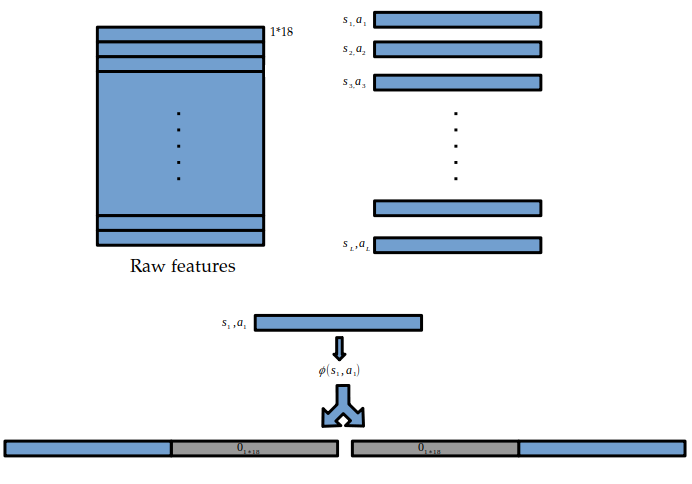
\includegraphics[scale=.40]{phi.png}
	  \label{fig:phi}
	\end{figure}
\end{frame}
%=====================================%
%=====================================%

\begin{frame}
	\frametitle{Evaluation}
	\begin{itemize}
		\item Two tests:
		\begin{itemize}
			\item The bigger set to train the system, and small set to test
			\item The bigger set used as the input for a k-fold cross validation, choosing k, and test on the small data set
		\end{itemize}
		\item Bellman Error is used for evaluation
		\begin{equation}
		\begin{split}
		 BE^\pi & =(TQ^\pi) - Q^\pi \\
		 & = R + \gamma \phi(s',a') w - \phi(s,a) w 
		\end{split}
		\end{equation}
	\end{itemize}
	\begin{center} \label{tab:be}
	\begin{tabular}{ |c|c| } 
	 \hline
	 Method & BE \\ 
	 \hline
	 LSTDQ & 4935580.30 \\ 
	 LSTDQ with 4-fold & 4905981.01 \\ 
	 LSTDQ with 5-fold & 4601911.70 \\ 
	 LSTDQ with 6-fold & 4919249.69 \\ 
	 LSTDQ with 10-fold& 4886872.99 \\
	 \hline
	\end{tabular}
	\end{center}
\end{frame}
%=====================================%
%=====================================%

\begin{frame}
	\frametitle{Results}
	\begin{figure}
	  \centering
	  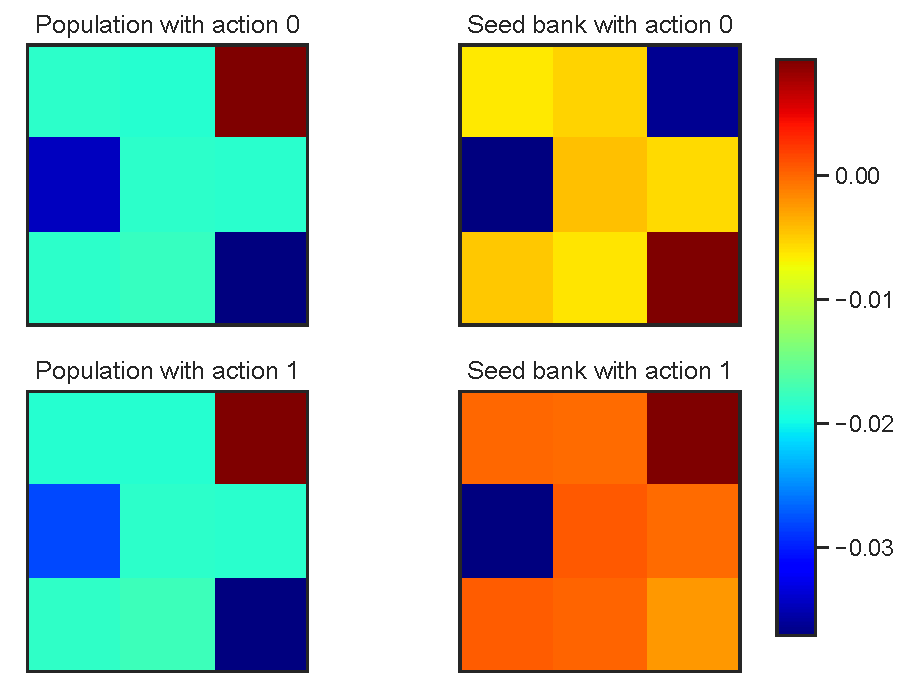
\includegraphics[scale=.40]{Ew.pdf}
	  \label{fig:ew}
	\end{figure}
\end{frame}
%=====================================%
% %=====================================%

% \begin{frame}
% 	\frametitle{Background}
% 	\begin{itemize}

% 	\end{itemize}
% \end{frame}
% %=====================================%



%=====================================%

% \begin{frame}
% 	\begin{center}
% 		\Huge Thank You!
% 	\end{center}
% \end{frame}
%=====================================%

% \begin{frame}
	% \frametitle{Background}
% 	\begin{itemize}
% 		\item 
% 	\end{itemize}
% \end{frame}


\end{document}
